\chapter{AIX}
\section{Introducci\'on}
AIX ({\it Advanced Interactive eXecutive}) es la versi\'on de Unix desarrollada 
y mantenida desde hace m\'as de diez
a\~nos por IBM; sus or\'{\i}genes provienen de IBM RT System, de finales de los 
ochenta, y se ejecuta en las plataformas RS/6000, basadas en {\it chips} {\sc 
risc} PowerPC similares al utilizados por algunos Macintosh m\'as o menos 
modernos. Este operativo, mezcla de {\sc bsd} y {\it System V} (se suele decir
que no es ni uno ni otro) es el que m\'as caracter\'{\i}sticas propietarias 
incorpora, caracter\'{\i}sticas que no se encuentran en ninguna otra versi\'on 
de Unix, por lo que a cualquier administrador le costar\'a m\'as adaptarse a 
AIX que a otros Unices. No obstante, en favor de IBM hay que decir que dispone
de un excelente asistente para realizar todo tipo de tareas denominado {\sc 
smit} ({\it System Management Interface Tool}, tambi\'en ejecutado como {\tt 
smitty} en modo consola): aunque por supuesto cualquier tarea tambi\'en se 
puede ejecutar desde la l\'{\i}nea de comandos, esto generalmente no se hace 
con las \'ordenes habituales de Unix, por lo que {\sc smit} es una herramienta
indispensable para el administrador de la m\'aquina. AIX, a pesar de que en un 
principio pueda parecer el Unix m\'as arcaico -- y nadie niega que lo sea -- es 
un entorno de trabajo fiable y sobre todo extremadamente estable, e incluso 
incorpora caracter\'{\i}sticas (tanto de seguridad como de otros aspectos) que 
ya quisieran para s\'{\i} otros sistemas Unix.\\
\\El hecho de que muchas tareas no se realicen en AIX de la misma forma en que 
se llevan a cabo en el resto de Unices es en parte debido al {\sc odm} ({\it
Object Data Manager}); a diferencia de Solaris o Linux, en AIX debemos tener
presente en todo momento que {\tt vi} {\bf no} es una herramienta para 
administrar el sistema, ya que los cl\'asicos ficheros de configuraci\'on {\sc 
ASCII} han sido sustituidos por archivos binarios, bases de datos que mantienen
la configuraci\'on del sistema (aspectos como los dispositivos, los recursos 
del entorno, o el subsistema de comunicaciones de AIX) de forma m\'as robusta, 
segura y portable que los simples ficheros de texto, al menos en opini\'on de 
los desarrolladores de IBM (\cite{kn:bet00}).\\
\\IBM mantiene en Internet un excelente repositorio de documentaci\'on,
principalmente los denominados {\it RedBooks}, completos manuales sobre casi 
cualquier tema relacionado con AIX -- y otros productos de la compa\~n\'{\i}a --
que podamos imaginar. Est\'an disponibles en la direcci\'on {\tt 
http://www.redbooks.ibm.com/}, y algunos de ellos son una herramienta 
imprescindible para cualquier administrador de sistemas. Por supuesto, 
tambi\'en es muy recomendable instalar las p\'aginas del manual {\it on--line}
de AIX, algo que incomprensiblemente no se hace por defecto en una instalaci\'on
est\'andar, y utilizar {\sc smit} para ejecutar cualquier tarea que desde 
l\'{\i}nea de \'ordenes dudemos de c\'omo hacer.\\
\\En este cap\'{\i}tulo hablaremos de aspectos de la seguridad casi exclusivos
de AIX; al ser este sistema probablemente el Unix m\'as cerrado de todos, lo
que veamos aqu\'{\i} dif\'{\i}cilmente ser\'a extrapolable -- en la mayor\'{\i}a
de casos -- a otros entornos como Solaris o HP--UX. En cualquier caso, es
necesario para un administrador conocer los aspectos de AIX que le confieren su
enorme robustez, tanto en lo referente a seguridad como en cualquier otra faceta
gen\'erica del sistema.
\section{Seguridad f\'{\i}sica en RS/6000}
El {\it firmware} de los sistemas RS/6000 provee de tres modos de protecci\'on
f\'{\i}sica (\cite{kn:ibm00}), en cierta forma similares a las que ofrecen las 
estaciones {\sc
sparc} que comentamos al hablar de Solaris. El primero de ellos, denominado 
{\sc pop} ({\it Power--On Password}) es el equivalente al modo {\tt 
`full-secure'} de {\sc sparc}, y como \'este impide el arranque del sistema si 
antes no se ha introducido la contrase\~na determinada como {\sc pop}; por
supuesto, esto evita tareas como la planificaci\'on de reinicios autom\'aticos,
por lo que en muchas ocasiones no compensa el nivel de seguridad con el de
funcionalidad. Por eso existe un segundo modo de protecci\'on denominado {\it
Unattended start mode} que permite arrancar al sistema de su dispositivo por
defecto sin necesidad de que un operador teclee la contrase\~na {\sc pop} para
ello.\\
\\En el modo `desatendido' el sistema arranca con normalidad desde el 
dispositivo especificado por defecto sin necesidad de ninguna clave {\sc pop} 
(a pesar de que esta contrase\~na tenga que haber sido definida con 
anterioridad); el sistema arranca, pero la diferencia con el modo normal es que 
el controlador de teclado permanece bloqueado hasta el el {\it password} {\sc 
pop} es introducido. De esta forma se consigue que la m\'aquina proporcione 
todos sus servicios (el arranque es completo) pero que, si alguien quiere 
acceder a la misma desde consola, est\'e obligado a introducir la contrase\~na
{\sc pop} previamente definida.\\
\\Aparte del {\it password} {\sc pop}, en las m\'aquinas RS/6000 puede 
establecerse una segunda contrase\~na denominada {\sc pap} ({\it Privileged
Access Password}) o {\it Supervisory Password}, que protege el arranque del 
{\sc sms} 
({\it System Management Services}), un {\it firmware} que proporciona al
administrador de la m\'aquina ciertas utilidades de configuraci\'on de bajo 
nivel; el {\sc sms} es accesible en un determinado punto de la secuencia de
arranque de la m\'aquina, en concreto cuando el {\it display} marca {\sc `ff1'} 
y se pulsa una cierta tecla (generalmente {\tt `1'} en terminales de texto o 
{\sc `f1'} en terminales gr\'aficas), y desde sus men\'us se puede actualizar el
propio {\it firmware} o cambiar el dispositivo de arranque, por poner s\'olo un
par de ejemplos. Si la contrase\~na {\sc pap} est\'a habilitada se restringe el 
acceso al {\sc sms}, evitando que 
un atacante con acceso f\'{\i}sico al equipo puede modificar par\'ametros de la
m\'aquina vitales para nuestra seguridad.\\
\\Es importante establecer un {\it password} para proteger el {\sc sms}: si un
pirata consigue acceso al mismo, ni tan siquiera importar\'a si hemos definido 
o no
una contrase\~na {\sc pop}, ya que podr\'a deshabilitarla o incluso cambiarla
desde el {\sc sms}; el problema surge si la clave de nuestro {\it firmware} se
pierde, ya que en ese caso necesitar\'{\i}amos abrir el equipo y quitarle su
bater\'{\i}a, perdiendo en este caso toda la configuraci\'on almacenada en la
{\sc nvram}.\\
\\Desde la l\'{\i}nea de \'ordenes de un sistema AIX podemos ejecutar ciertos
mandatos que nos van a permitir tanto visualizar el valor de par\'ametros del 
{\it firmware} como modificar dicho valor; lamentablemente no tenemos un 
interfaz tan uniforme como en Solaris, donde a trav\'es de la orden {\tt 
eeprom} leemos y modificamos la informaci\'on de la {\sc nvram}, sino que en AIX
tenemos que utilizar diferentes \'ordenes para interactuar con el {\it 
firmware} de la m\'aquina. Por ejemplo, mediante un comando como {\tt bootlist}
podemos consultar y modificar la lista de dispositivos de arranque del sistema,
y mediante {\tt lscfg} obtener la versi\'on del {\it firmware} instalado en la
m\'aquina:
\begin{quote}
\begin{verbatim}
bruja:/# bootlist -m normal -o
hdisk0
fd0
cd0
ent2
bruja:/#
\end{verbatim}
\end{quote}
\section{Servicios de red}
Como en el resto de entornos Unix, en AIX es vital garantizar la seguridad de
los servicios de red de la m\'aquina para conseguir un entorno de trabajo 
fiable en su globalidad; no obstante, este operativo provee de una serie de 
herramientas que otros sistemas no proporcionan y que facilitan enormemente el
trabajo del administrador: es importante acostumbrarse a su manejo (recordemos
que en AIX {\tt vi} {\bf no} es una herramienta administrativa) a trav\'es de
{\sc smit} y, mucho mejor, desde l\'{\i}nea de \'ordenes. Por poner un ejemplo,
si a un administrador de un entorno Solaris, Linux o HP-UX le preguntamos 
c\'omo eliminar\'{\i}a el servicio {\tt chargen} en una m\'aquina, la respuesta
ser\'{\i}a siempre la misma: editando {\tt /etc/inetd.conf}, comentando la
l\'{\i}nea correspondiente con una almohadilla ({\tt `\#'}) y reiniciando el
demonio {\tt inetd} envi\'andole la se\~nal {\sc sighup}; si le preguntamos lo
mismo al {\tt root} de una m\'aquina AIX, lo m\'as probable (aunque podr\'{\i}a
hacerlo de la forma anterior) es que utilice una orden como {\tt chsubserver}, 
en un proceso similar al siguiente:
\begin{quote}
\begin{verbatim}
bruja:/# grep chargen /etc/inetd.conf
chargen        stream  tcp     nowait  root    internal
chargen        dgram   udp     wait    root    internal
bruja:/# chsubserver -d -v chargen -p udp
bruja:/# chsubserver -d -v chargen -p tcp
bruja:/# grep chargen /etc/inetd.conf
#chargen        stream  tcp     nowait  root    internal
#chargen        dgram   udp     wait    root    internal
bruja:/# refresh -s inetd
bruja:/#
\end{verbatim}
\end{quote}
En AIX los subsistemas de red son gestionados por el Controlador de Recursos del
Sistema ({\sc src}, {\it System Resource Controller}), un {\it software} que
proporciona comandos e interfaces uniformes para crear y controlar {\bf 
subsistemas} (\cite{kn:ibm97}), que no son m\'as que programas o procesos (o
combinaciones de los mismos) capaces de operar de forma independiente o a 
trav\'es de un controlador, algo que es m\'as o menos equivalente a lo que 
todos conocemos como `demonio' en cualquier Unix; podemos ejecutar la orden 
{\tt `lssrc -a'} para listar los subsistemas de nuestra m\'aquina AIX:
\begin{quote}
\begin{verbatim}
bruja:/# lssrc -a
Subsystem         Group            PID     Status 
 portmap          portmap          5684    active
 inetd            tcpip            7770    active
 xntpd            tcpip            6352    active
 automountd       autofs           6056    active
 hats             hats             9876    active
 hags             hags             8494    active
 hagsglsm         hags             9370    active
 haem             haem             6694    active
 haemaixos        haem             10662   active
 pman             pman             11372   active
 pmanrm           pman             12130   active
 sysctld                           11174   active
 snmpd            tcpip            15520   active
 sendmail         mail             16628   active
 dpid2            tcpip            16106   active
 fs                                19612   active
 biod             nfs              19874   active
 rpc.statd        nfs              20644   active
 qdaemon          spooler          15750   active
 writesrv         spooler          19366   active
 clstrmgr         cluster          32706   active
 clsmuxpd         cluster          42048   active
 nfsd             nfs              31168   active
 rpc.mountd       nfs              42904   active
 rpc.lockd        nfs              32004   active
 tftpd            tcpip            7586    active
 syslogd          ras              31852   active
 lpd              spooler                  inoperative
 clvmd                                     inoperative
 gated            tcpip                    inoperative
 named            tcpip                    inoperative
 routed           tcpip                    inoperative
 rwhod            tcpip                    inoperative
 iptrace          tcpip                    inoperative
 timed            tcpip                    inoperative
 dhcpcd           tcpip                    inoperative
 dhcpsd           tcpip                    inoperative
 dhcprd           tcpip                    inoperative
 ndpd-host        tcpip                    inoperative
 ndpd-router      tcpip                    inoperative
 llbd             iforncs                  inoperative
 glbd             iforncs                  inoperative
 i4lmd            iforls                   inoperative
 i4glbcd          iforncs                  inoperative
 i4gdb            iforls                   inoperative
 i4llmd           iforls                   inoperative
 mrouted          tcpip                    inoperative
 rsvpd            qos                      inoperative
 policyd          qos                      inoperative
 pxed             tcpip                    inoperative
 binld            tcpip                    inoperative
 dtsrc                                     inoperative
bruja:/# 
\end{verbatim}
\end{quote}
\begin{figure}
\begin{center}
\setlength{\unitlength}{3947sp}%
%
\begingroup\makeatletter\ifx\SetFigFont\undefined%
\gdef\SetFigFont#1#2#3#4#5{%
  \reset@font\fontsize{#1}{#2pt}%
  \fontfamily{#3}\fontseries{#4}\fontshape{#5}%
  \selectfont}%
\fi\endgroup%
\begin{picture}(6324,2424)(-11,-1648)
\thinlines
\put(976,314){\framebox(975,300){}}
\put(301,-286){\framebox(2625,300){}}
\put(676,-1486){\framebox(1725,300){}}
\put(826,-886){\framebox(1425,300){}}
\put(1426,314){\vector( 0,-1){300}}
\put(1426,-286){\vector( 0,-1){300}}
\put(1426,-886){\vector( 0,-1){300}}
\put(  1,-1636){\framebox(6300,2400){}}
\put(376,-211){\makebox(0,0)[lb]{\smash{\SetFigFont{12}{14.4}{\sfdefault}{\mddefault}{\updefault}GRUPOS DE SUBSISTEMAS}}}
\put(1051,389){\makebox(0,0)[lb]{\smash{\SetFigFont{12}{14.4}{\sfdefault}{\mddefault}{\updefault}SISTEMA}}}
\put(751,-1411){\makebox(0,0)[lb]{\smash{\SetFigFont{12}{14.4}{\sfdefault}{\mddefault}{\updefault}SUBSERVIDORES}}}
\put(901,-811){\makebox(0,0)[lb]{\smash{\SetFigFont{12}{14.4}{\sfdefault}{\mddefault}{\updefault}SUBSISTEMAS}}}
\put(4051,389){\makebox(0,0)[lb]{\smash{\SetFigFont{14}{16.8}{\ttdefault}{\mddefault}{\updefault}(bruja)}}}
\put(3976,-211){\makebox(0,0)[lb]{\smash{\SetFigFont{14}{16.8}{\ttdefault}{\mddefault}{\updefault}(tcpip)}}}
\put(3976,-811){\makebox(0,0)[lb]{\smash{\SetFigFont{14}{16.8}{\ttdefault}{\mddefault}{\updefault}(inetd)}}}
\put(3526,-1411){\makebox(0,0)[lb]{\smash{\SetFigFont{14}{16.8}{\ttdefault}{\mddefault}{\updefault}(telnetd, ftpd...)}}}
\end{picture}
\end{center}
\caption{Estructura jer\'arquica del {\sc src}.}
\label{subsystem}
\end{figure}
Los subsistemas con funciones relacionadas entre s\'{\i} forman lo que se 
denomina {\bf grupos de subsistemas}, y adem\'as cada subsistema se divide en 
{\bf subservidores} (simples programas o procesos), formando una estructura
jer\'arquica como la mostrada en la figura \ref{subsystem} (figura en la que
adem\'as se muestra un ejemplo -- entre par\'entesis -- de cada categor\'{\i}a);
como podemos ver en ella, un grupo de subsistemas es {\tt tcpip}, que como su
nombre ya adelanta es el encargado de la gesti\'on de protocolos {\sc tcp/ip}, 
y que incluye a subsistemas tan importantes como {\tt inetd} o {\tt snmpd}. 
Mediante {\tt lssrc}, con las opciones adecuadas, podemos obtener informaci\'on 
detallada acerca de un subsistema o subservidor; por ejemplo, la siguiente 
orden nos muestra lo que hemos comentado anteriormente, que el subsistema {\tt 
inetd} pertenece al grupo {\tt tcpip}, y que en este caso concreto tiene
cuatro servidores activos ({\tt tftp}, {\tt klogin}, {\tt kshell} y {\tt ftp}):
\begin{quote}
\begin{verbatim}
bruja:/# lssrc -ls inetd
Subsystem         Group            PID     Status 
 inetd            tcpip            7770    active
  
Debug         Not active 
  
Signal        Purpose 
 SIGALRM      Establishes socket connections for failed services. 
 SIGHUP       Rereads the configuration database and reconfigures services. 
  
 SIGCHLD      Restarts the service in case the service ends abnormally. 
  
Service       Command                  Description              Status 
 tftp         /usr/sbin/tftpd          tftpd -d /tftpboot       active
 klogin       /usr/sbin/krlogind       krlogind                 active
 kshell       /usr/sbin/krshd          krshd                    active
 ftp          /usr/sbin/ftpd           ftpd                     active
  
bruja:/#
\end{verbatim}
\end{quote}
Como ya hemos dicho antes, el {\sc src} proporciona comandos comunes para
operar con todos sus subsistemas: disponemos de las \'ordenes {\tt startsrc} y 
{\tt stopsrc} para arrancar y detener -- respectivamente -- tanto subsistemas 
completos como subservidores de los mismos de forma independiente, y de {\tt 
traceson} y {\tt tracesoff} para activar o desactivar el trazado de los mismos;
la orden {\tt refresh} `refresca' un subsistema (algo similar a enviarle una 
se\~nal {\sc sighup}), mientras que mediante {\tt lssrc} podemos consultar el 
estado de un subsistema. Por ejemplo, para detener el subservidor {\tt telnetd} 
en nuestro sistema no tenemos que recurrir -- aunque podr\'{\i}amos hacerlo --
a {\tt chsubserver} (como vimos al inicio de este punto aplicando el ejemplo al
subservidor {\tt chargen}); una forma equivalente de hacerlo es simplemente 
ejecutando la siguiente orden:
\begin{quote}
\begin{verbatim}
bruja:/# startsrc -t telnet
0513-124 The telnet subserver has been started.
bruja:/# grep -w telnet /etc/inetd.conf
telnet  stream  tcp6    nowait  root    /usr/sbin/telnetd      telnetd -a
bruja:/# stopsrc -t telnet
0513-127 The telnet subserver was stopped successfully.
bruja:/# grep -w telnet /etc/inetd.conf
#telnet  stream  tcp6    nowait  root    /usr/sbin/telnetd      telnetd -a
bruja:/# 
\end{verbatim}
\end{quote}
\section{Usuarios y accesos al sistema}
Como vamos a ver en esta secci\'on, AIX ofrece un sistema de control de accesos 
y gesti\'on de usuarios realmente interesante; al igual que en cualquier entorno
Unix, nada m\'as instalar el operativo ya existen una serie de usuarios `del
sistema' ({\tt root}, {\tt daemon}, {\tt sys}\ldots). Todos ellos tienen en 
realidad las cuentas bloqueadas ya que el campo reservado a su contrase\~na en
{\tt /etc/security/passwd} es un asterisco, aunque una orden como {\tt
`lsuser'} nos diga lo contrario: 
\begin{quote}
\begin{verbatim}
bruja:/# lsuser -a account_locked ALL
root account_locked=false 
daemon account_locked=false 
bin account_locked=false 
sys account_locked=false 
adm account_locked=false 
uucp account_locked=false 
guest account_locked=false 
nobody account_locked=false 
lpd account_locked=false
imnadm account_locked=false 
nuucp account_locked=false 
bruja:/#
\end{verbatim}
\end{quote}
Si necesitamos que la cuenta de un determinado usuario se bloquee temporalmente
pero no queremos sustituir su clave del fichero de contrase\~nas por un
asterisco, podemos ejecutar
la orden {\tt `chuser'}\footnote{Es necesario recordar una vez m\'as que en 
AIX, a diferencia de otros Unices, {\tt vi} {\bf no es ninguna herramienta 
administrativa}.}:
\begin{quote}
\begin{verbatim}
bruja:/# lsuser -a account_locked toni
toni account_locked=false 
bruja:/# chuser account_locked=true toni
bruja:/# lsuser -a account_locked toni
toni account_locked=true 
bruja:/# 
\end{verbatim}
\end{quote}
La gesti\'on y el control de los accesos al sistema por parte de usuarios se
puede llevar a cabo desde diferentes ficheros del directorio {\tt 
/etc/security/}: por ejemplo, en el archivo {\tt user} se definen los diferentes
atributos de cada usuario del sistema, desde las propiedades de envejecimiento
de su contrase\~na a las franjas horarias en que el usuario pueden acceder a 
la m\'aquina; vamos a ver en los siguientes puntos algunos de estos archivos,
interesantes para definir o refinar par\'ametros relacionados con la seguridad
de nuestro sistema.
\subsection{El fichero {\tt /etc/security/.ids}}
El nombre de este archivo quiz\'as nos puede inducir a pensar que se trata de
algo relacionado con la detecci\'on de intrusos en nuestra m\'aquina; nada
m\'as lejos de la realidad: en el fichero {\tt .ids} se almacena informaci\'on
necesaria para generar correctamente a nuevos usuarios. Su formato es similar 
al siguiente:
\begin{quote}
\begin{verbatim}
bruja:/etc/security# cat .ids
8 210 11 205
bruja:/etc/security#
\end{verbatim}
\end{quote}
Donde {\tt `8'} y {\tt `11'} indican los siguientes {\sc uid} y {\sc gid}
(respectivamente) disponibles para usuarios con privilegios administrativos,
mientras que {\tt `210'} y {\tt `205'} son equivalentes pero para usuarios sin
dichos privilegios.\\
\\A no ser que conozcamos muy bien el sistema, no es recomendable modificar 
manualmente este archivo, ya que las herramientas de gesti\'on de usuarios lo 
actualizan de forma autom\'atica; de cualquier forma, aqu\'{\i} lo citamos para 
evitar confusiones con su nombre, como hemos comentado al principio.
\subsection{El fichero {\tt /etc/security/passwd}}
Al contrario de lo que sucede con el archivo {\tt .ids}, el nombre del fichero 
{\tt passwd} no da lugar a equivocaciones: se trata, evidentemente, de 
informaci\'on sobre las claves de los usuarios del sistema. Esta informaci\'on
puede estar desajustada con respecto a la contenida en {\tt /etc/passwd}, por
lo que es recomendable ejecutar peri\'odicamente -- al menos una vez al mes --
\'ordenes como {\tt pwdck}, {\tt usrck} o {\tt grpck}, encargadas de verificar, 
comparar y sincronizar la informaci\'on de los usuarios (definiciones, grupos y
autenticaci\'on) en las diferentes tablas que AIX mantiene:
\begin{quote}
\begin{verbatim}
bruja:/# pwdck -y ALL
The user "daemon" has an invalid password field in /etc/passwd.
The user "toni" has an invalid password field in /etc/passwd.
bruja:/# usrck -n ALL
User daemon is locked.
User bin is locked.
User sys is locked.
User nobody is locked.
User lpd is locked.
User imnadm is locked.
bruja:/# 
\end{verbatim}
\end{quote}
Tras sincronizar correctamente la informaci\'on de los usuarios (par\'ametro
{\tt `-y'} de estas \'ordenes), en {\tt /etc/passwd} nos encontraremos el
car\'acter {\tt `!'} en el campo reservado a la contrase\~na cifrada de cada 
entrada, mientras que las claves reales ya estar\'an en {\tt 
/etc/security/passwd}. Este fichero ha de ser de s\'olo lectura para el 
administrador: es en cierta forma similar al {\tt /etc/shadow} cl\'asico de 
otros Unices; no obstante, difiere enormemente de \'el en el formato del 
archivo, ya que no utiliza una entrada por l\'{\i}nea con los campos separados 
por el car\'acter {\tt `:'}. Por contra, en AIX cada usuario tiene definidos
una serie de campos, uno por l\'{\i}nea, y con el identificador del campo y su
contenido separados por un signo {\tt `='}; por ejemplo, la entrada para el
usuario {\tt `oracle'} en {\tt /etc/security/passwd} podr\'{\i}a ser similar a
la siguiente:
\begin{quote}
\begin{verbatim}
oracle:
        password = be3a2NjB.dtbg
        lastupdate = 995301219
        flags = 
\end{verbatim}
\end{quote}
El primer campo representa obviamente la contrase\~na cifrada del usuario;
el segundo representa el la fecha y hora de la \'ultima actualizaci\'on del
conjunto de atributos (denominado {\it `stanza'}) del usuario, y finalmente el
campo {\tt `flags'}, por defecto vac\'{\i}o, puede contener una serie de
par\'ametros caracter\'{\i}sticos del usuario concreto: si se trata de un
usuario con cierto privilegio, si no necesita contrase\~na para conectar al
sistema\ldots; para obtener m\'as informaci\'on sobre estos par\'ametros 
podemos consultar la p\'agina del manual de {\tt `pwdck'}.
\subsection{El fichero {\tt /etc/security/failedlogin}}
Como su nombre indica, en este fichero se registran los intentos fallidos de
acceso al sistema; su formato no es de texto plano, sino que es similar a
los ficheros {\tt wtmp} de AIX y otros sistemas Unix. Por tanto, para 
visualizar el contenido de este archivo necesitamos ejecutar \'ordenes como 
{\tt `last'} o {\tt `who'} con los par\'ametros adecuados:
\begin{quote}
\begin{verbatim}
bruja:/# who -s /etc/security/failedlogin |tail -3
oracle      pts/24      Sep  5 12:55    (luisa)
UNKNOWN_    dtlogin/_0  Sep 12 11:01                    
toni        pts/23      Sep 13 15:45    (anita)
bruja:/# 
\end{verbatim}
\end{quote}
\subsection{El fichero {\tt /etc/security/lastlog}}
En el archivo {\tt /etc/security/lastlog} de un sistema AIX, un fichero de
texto plano que poco tiene que ver con el formato del {\tt `lastlog'} de otros 
Unices, se encuentra almacenada informaci\'on relativa a la \'ultima 
conexi\'on -- o intento de conexi\'on -- de cada usuario de la m\'aquina; en
concreto, aparecen referencias a la hora, terminal y {\it host} origen de la
\'ultima entrada al sistema y del \'ultimo intento de acceso.\\
\\Cuando un usuario es creado mediante {\tt mkuser} (o equivalentemente, 
v\'{\i}a {\sc smit}) se crea una {\it stanza} vac\'{\i}a para el mismo en este 
archivo cuyos campos se ir\'an rellenando a medida que el usuario acceda al
sistema; esta {\it stanza} puede ser similar a la siguiente:
\begin{quote}
\begin{verbatim}
toni:
        time_last_login = 1005297794
        tty_last_login = ttyp0           
        host_last_login = anita
        unsuccessful_login_count = 0         
        time_last_unsuccessful_login = 1004445794
        tty_last_unsuccessful_login = /dev/pts/14     
        host_last_unsuccessful_login = luisa
\end{verbatim}
\end{quote}
Como podemos ver, el nombre de cada campo es autoexplicativo de su funci\'on; el
\'unico que quiz\'as puede plantear alguna duda es {\tt 
unsuccessful$\_$login$\_$count}, que no es m\'as que un contador que indica el
n\'umero de intentos de acceso fallidos desde la \'ultima entrada al sistema.\\
\\Para consultar los par\'ametros de cada usuario almacenados en este archivo
no es necesario editar o visualizar el fichero: mediante la orden {\tt lsuser}
podemos obtener el valor de cada uno de ellos; si por ejemplo nos interesa
el nombre de la m\'aquina desde la que el usuario {\tt toni} accedi\'o por
\'ultima vez al sistema, podemos conseguirlo de esta forma:
\begin{quote}
\begin{verbatim}
bruja:/# lsuser -a host_last_login toni
toni host_last_login=anita
bruja:/# 
\end{verbatim}
\end{quote}
\subsection{El fichero {\tt /etc/security/limits}}
En este archivo se definen l\'{\i}mites a algunos de los recursos que ofrece un
entorno de trabajo AIX; como muchos de los archivos del directorio, contiene
una {\it stanza} que se aplica por defecto y luego entradas -- vac\'{\i}as por 
lo general -- para cada usuario, en las que se pueden personalizar par\'ametros 
que s\'olo se aplican a uno o varios usuarios y no a todos (generalmente se 
definen al crear al usuario). Las diferentes directivas del archivo son las
siguientes: 
\begin{itemize}
\item {\tt fsize}\\
Tama\~no m\'aximo de un archivo en bloques de 512 {\it bytes}.
\item {\tt core}\\
Tama\~no m\'aximo de un fichero {\tt core} (volcado de memoria) en bloques de 
512 {\it bytes}.
\item {\tt cpu}\\
Tiempo l\'{\i}mite de CPU por proceso, especificado en segundos. Por defecto no
est\'a establecido para ning\'un usuario.
\item {\tt data}\\
L\'{\i}mite de tama\~no del segmento de datos de un proceso del usuario, en 
bloques de 512 {\it bytes}.
\item {\tt stack}\\
L\'{\i}mite de tama\~no de la pila de un proceso en bloques de 512 {\it bytes}.
\item {\tt rss}\\
L\'{\i}mite del tama\~no de memoria utilizada por proceso, en bloques de 512 
{\it bytes}.
\item {\tt nofiles}\\
N\'umero m\'aximo de descriptores de fichero abiertos.
\end{itemize}
Cada uno de los l\'{\i}mites anteriores es un l\'{\i}mite {\it soft} (blando)
que el usuario puede sobrepasar si lo desea, modificando su valor mediante 
la orden {\tt ulimit}; existen, definidos en el mismo archivo, l\'{\i}mites {\it
hard} (duros) que el usuario no puede incrementar de ninguna forma. El nombre
de cada uno de ellos es el mismo que el de su equivalente {\it soft} pero 
a\~nadi\'endole la coletilla {\tt `$\_$hard'}: {\tt fsize$\_$hard}, {\tt 
rss$\_$hard},etc.\\
\\Podemos ver los l\'{\i}mites aplicables a uno o m\'as usuarios mediante la 
orden {\tt `lsuser'} (un valor de `-1' indica que se trata de un recurso no
limitado al usuario en cuesti\'on):
\begin{quote}
\begin{verbatim}
bruja:/# lsuser -f -a fsize core cpu data stack rss nofiles toni
toni:
        fsize=2097151
        core=2097151
        cpu=-1
        data=262144
        stack=65536
        rss=65536
        nofiles=2000

bruja:/# 
\end{verbatim}
\end{quote}
Por defecto, AIX ofrece unos l\'{\i}mites bastante razonables a los recursos que
cada usuario puede consumir; no obstante, en funci\'on de para qu\'e se utilice
cada sistema concreto, es recomendable que sea el administrador el que deba 
especificar qu\'e limites impone a los usuarios sobre los recursos de la
m\'aquina para prevenir negaciones de servicio contra los mismos.
\subsection{El fichero {\tt /etc/security/login.cfg}}
En este archivo se definen ciertos par\'ametros de control para las conexiones
remotas a un sistema AIX; como veremos en este punto, todos ellos tienen
implicaciones directas, aunque de diferente grado, en la seguridad del entorno
de trabajo. Se puede dividir en tres grandes \'areas: la correspondiente a la
definici\'on de puertos, la relativa a m\'etodos de autenticaci\'on de usuarios
y la que define atributos tambi\'en de los usuarios; todas ellas contienen una
{\it stanza} por defecto, y adicionalmente definiciones particulares para 
elementos concretos.\\
\\La primera gran \'area del archivo, la relativa a los puertos, est\'a formada
por una serie de par\'ametros que definen caracter\'{\i}sticas del acceso al
sistema a trav\'es de ellos; la primera directiva de este grupo es {\tt 
herald}, que permite definir el
mensaje que se muestra en la pantalla del usuario que trata de establecer una
conexi\'on remota con el sistema (algo similar al archivo {\tt /etc/motd} del
resto de Unices, fichero que en AIX no existe -- y si es creado no tiene efecto 
--). Cuando tratamos de acceder a una m\'aquina AIX el mensaje que se muestra
es similar al siguiente:
\begin{quote}
\begin{verbatim}
luisa:~$ telnet bruja
Trying 192.168.0.10...
Connected to bruja.
Escape character is '^]'.


telnet (bruja)

AIX Version 4
(C) Copyrights by IBM and by others 1982, 1996.
login:  
\end{verbatim}
\end{quote}
Modificando la directiva {\tt herald} de {\tt /etc/security/login.cfg} podemos
definir otros mensajes de presentaci\'on; si por ejemplo queremos simular que
nuestra m\'aquina ejecuta Solaris en lugar de AIX, podemos emular el mensaje
del primero:
\begin{quote}
\begin{verbatim}
bruja:/# grep herald /etc/security/login.cfg
herald = "SunOS 5.8\n\nlogin: "
bruja:/# 
\end{verbatim}
\end{quote}
As\'{\i}, cuando un usuario trate de conectar al sistema, ver\'a algo parecido 
a lo siguiente:
\begin{quote}
\begin{verbatim}
bruja:/# telnet 0
Trying...
Connected to 0.
Escape character is '^]'.

SunOS 5.8

login:^D Connection closed.
bruja:/#
\end{verbatim}
\end{quote}
Relacionada con el anterior par\'ametro tenemos la directiva {\tt herald2}, 
formada por una cadena de texto y que define el mensaje de {\it login} impreso
en la terminal tras un intento fallido de acceso al sistema; por defecto, esta
cadena de texto es un nuevo {\it prompt} de {\it login}.\\
\\Tambi\'en relativa a los puertos, otra directiva interesante que podemos 
encontrar en el fichero {\tt login.cfg}
es {\tt logindelay}, que permite especificar el retardo en segundos entre
intentos consecutivos de entrada al sistema; si es diferente de 0 (si es 0 se
deshabilita su efecto) el valor de este par\'ametro se multiplica por el 
n\'umero de intentos fallidos: si {\tt logindelay} es 1 el retardo entre el 
primer y el segundo intento ser\'a de un segundo, entre el segundo y el tercero
ser\'a de dos, etc. Junto a este par\'ametro podemos definir tambi\'en la
directiva {\tt logindisable}, que marca el n\'umero de intentos de entrada al
sistema fallidos que una conexi\'on acepta antes de cerrarse -- o bloquearse, si
se trata de una l\'{\i}nea serie --, {\tt logininterval}, que define los 
segundos durante los que se tienen que producir los intentos fallidos de 
conexi\'on para que se cierre o bloquee la misma, y {\tt loginreenable}, que
obviamente indica el intervalo -- en minutos -- que un puerto va a permanecer
bloqueado (si su valor es 0 -- y por defecto lo es -- estar\'a as\'{\i} hasta 
que el administrador lo desbloquee manualmente mediante {\tt chsec}).\\
\\Otra entrada \'util en el archivo {\tt login.cfg} es {\tt logintimes}, que
como su nombre indica define las horas y d\'{\i}as durante las que un puerto
determinado puede ser utilizado para acceder al sistema, algo similar (en idea, 
no en sintaxis) al archivo 
{\tt /etc/porttime} de Linux o al {\tt prot.pwd.DB} de HP-UX 10.x. El formato
utilizado para especificar los intervalos de horas o d\'{\i}as en los que el
acceso se permite (entradas llamadas {\sc allow}) o se deniega (entradas {\sc
deny}) no es inmediato, por lo que es recomendable -- como siempre en Unix -- 
consultar la p\'agina del manual de {\tt login.cfg}. Por defecto, se permite a
todos los usuarios acceder a trav\'es de cualquier l\'{\i}nea sin importar el
d\'{\i}a ni la hora.\\
\\Para finalizar con el \'area de puertos vamos a comentar un par de directivas
que tambi\'en se pueden definir en el archivo {\tt login.cfg}: se trata de
{\tt sak$\_$enabled} y {\tt synonym}. La primera de ellas indica si el {\it
secure attention key} ({\sc sak}) est\'a habilitado en el puerto, lo que implica
que los usuarios pueden obtener una ruta de comunicaci\'on fiable ({\it trusted 
communication path}, {\sc tcp}) mediante la combinaci\'on de teclas {\tt 
Ctrl-X} {\tt Ctrl-R}; en la secci\'on dedicada a la base fiable de c\'omputo de
los sistemas Unix ya hablamos de este tipo de comunicaciones seguras, por lo que
no vamos a entrar aqu\'{\i} en m\'as detalles. La segunda de las directivas a 
las que hac\'{\i}amos referencia, la denominada {\tt synonym}, tiene como 
objetivo definir sin\'onimos para una terminal concreta; est\'a bastante 
relacionada con la primera, ya que restringe el acceso al puerto, que s\'olo se
utilizar\'a para establecer una ruta de comunicaci\'on fiable con el sistema.\\
\\La segunda gran \'area del fichero {\tt /etc/security/login.cfg} hace 
referencia, como dijimos al principio, a los m\'etodos de autenticaci\'on de 
usuarios disponibles en la m\'aquina. M\'as tarde, cuando hablemos del fichero
{\tt /etc/security/user}, veremos que se pueden definir mecanismos secundarios
de autenticaci\'on en el sistema que funcionan de forma independiente o junto
al esquema cl\'asico de nombre de usuario y contrase\~na. Los programas que
implanten estos mecanismos adicionales han de definirse dentro de una {\it 
stanza}, bajo la directiva {\tt `program'}, que le de un nombre al modelo de 
autenticaci\'on que posteriormente se
definir\'a para uno o m\'as usuarios en {\tt /etc/security/user}; insistimos en
la palabra `adicionales', ya que los esquemas de autenticaci\'on cl\'asicos no
requieren definici\'on ({\sc system}, para acceder con nombre de usuario y
contrase\~na, y {\sc none}, para acceder sin autenticaci\'on). Por ejemplo, 
imaginemos que si queremos definir un nuevo m\'etodo basado en claves de un
solo uso al que vamos a denominar {\tt authone} y que est\'a implementado en el 
programa {\tt /usr/local/auth/onetime}; su {\it stanza} ser\'{\i}a similar a la
siguiente:
\begin{quote}
\begin{verbatim}
authone:
    program = /usr/local/auth/onetime
\end{verbatim}
\end{quote}
La \'ultima \'area del archivo proporciona la definici\'on de algunos 
atributos globales de los usuarios bajo una {\it stanza} \'unica: {\tt usw}. El
primero de estos atributos es {\tt logintimeout}, que define el tiempo en 
segundos (60, por defecto) que un usuario tiene para teclear su contrase\~na
cuando el sistema se lo solicita. Un segundo par\'ametro, {\tt maxlogins}, 
define el n\'umero m\'aximo de conexiones simult\'aneas que un usuario puede
abrir en el sistema: el valor por defecto, 100, es a todas luces excesivo en la
mayor parte de entornos, por lo que deber\'{\i}amos especificar un valor 
adecuado a nuestro sistema -- es imposible dar un valor `\'optimo' para esta
directiva --; si el valor de {\tt maxlogins} es 0, el n\'umero m\'aximo de 
conexiones simult\'aneas de un usuario est\'a ilimitado. Finalmente, el \'ultimo
par\'ametro, {\tt shells}, define los int\'erpretes de comandos v\'alidos en la 
m\'aquina, algo similar al archivo {\tt /etc/shells} de otros Unices. Una 
entrada t\'{\i}pica de esta {\it stanza} puede ser similar a la siguiente:
\begin{quote}
\begin{verbatim}
usw:
       shells = /bin/sh,/bin/bsh,/bin/csh,/bin/ksh,/bin/tsh,/usr/bin/sh
       maxlogins = 5
       logintimeout = 30
\end{verbatim}
\end{quote}
\subsection{El fichero {\tt /etc/security/user}}
En {\tt /etc/security/user} se definen atributos extendidos de cada usuario; 
dichos atributos no son m\'as que los no incluidos en el fichero {\tt 
/etc/passwd} convencional de todo sistema Unix: mientras que en este \'ultimo
encontramos datos como el {\it login} o el {\sc uid} de cada usuario, en el
primero tenemos informaci\'on como la fecha de caducidad de las contrase\~nas,
las horas a las que puede conectar cada usuario, o los requisitos de seguridad
m\'{\i}nimos para su clave. Cuando se a\~nade un usuario al sistema mediante 
la orden {\tt mkuser} se genera una nueva {\it stanza} en el fichero
correspondiente al nuevo usuario, con unos atributos por defecto tomados del
archivo {\tt /usr/lib/security/mkuser.default}; existen numerosos atributos 
extendidos para los usuarios, y conocer algunos de ellos es vital para 
incrementar los niveles de seguridad ofrecidos por defecto por AIX. En este 
punto vamos a hablar de estos atributos.\\
\\Una directiva b\'asica almacenada en {\tt /etc/security/user} es {\tt
account$\_$locked}, que evidentemente indica si una cuenta est\'a bloqueada o
no lo est\'a; es una variable booleana, por lo que sus posibles valores son 
sencillamente {\tt true} o {\tt false} (o equivalentemente, {\tt yes} y {\tt
always} o {\tt no} y {\tt never}). Aunque es muy similar a esta, la directiva
{\tt login} (tambi\'en booleana) no es exactamente igual: si su valor es {\tt
false} o equivalente el usuario no puede acceder al sistema, pero su cuenta no
est\'a bloqueada, ya que es posible llegar a ella mediante {\tt su}. Otra 
restricci\'on de acceso para un usuario viene determinada por {\tt rlogin}, que
define si un usuario puede acceder al sistema de forma remota a trav\'es de {\it
telnet} o {\tt rlogin} (otros m\'etodos de acceso, como {\sc ssh}, no son 
controlados por esta directiva).\\
\\El que un usuario no tenga su cuenta bloqueada ni su acceso deshabilitado 
implica que puede utilizar su
{\it login} para entrar -- evidentemente si su autenticaci\'on es correcta -- 
al sistema; algunas caracter\'{\i}sticas de este acceso tambi\'en se definen
en {\tt /etc/security/user}: por ejemplo, las horas y d\'{\i}as que un 
determinado usuario puede acceder al equipo, mediante la directiva {\tt 
logintimes} y las terminales desde las que puede hacerlo, mediante {\tt ttys}.
La sintaxis de la primera es equivalente a la utilizada en el fichero {\tt 
login.cfg}, pero afectando ahora a usuarios concretos y no a puertos, mientras
que la segunda se define mediante una lista de terminales separadas por comas;
alternativamente se pueden usar los comodines {\sc `all'} o {\tt `$\ast$'} para
indicar que el usuario puede acceder a trav\'es de cualquier l\'{\i}nea:
\begin{quote}
\begin{verbatim}
bruja:/# lsuser -a ttys toni
toni ttys=ALL
bruja:/#
\end{verbatim}
\end{quote}
Un grupo de directivas del archivo {\tt /etc/security/user} tambi\'en 
importantes para nuestra seguridad son las relativas a la contrase\~na de cada
usuario; una de ellas es {\tt expires}, que define la fecha de expiraci\'on de
la clave en formato {\sc mmddhhmmyy} (un cero, valor por defecto, indica que el 
{\it password} nunca caduca):
\begin{quote}
\begin{verbatim}
bruja:/# lsuser -a expires toni
toni expires=0
bruja:/#
\end{verbatim}
\end{quote}
Tambi\'en relacionada con el envejecimiento de claves tenemos la directiva
{\tt pwdwarntime}, que define el n\'umero de d\'{\i}as de antelaci\'on con los 
que se avisar\'a a un usuario antes de obligarle a cambiar su contrase\~na. El
periodo de validez de una clave viene indicado en semanas por la directiva {\tt 
maxage}, cuyo valor puede oscilar entre 0 (valor por defecto, que indica que no 
existe caducidad) o 52 (un a\~no de vida); por contra, el tiempo m\'{\i}nimo de 
vida de la contrase\~na se define en {\tt minage}, que puede tomar los mismos 
valores que la directiva anterior. Cuando una clave caduca entra en juego la
directiva {\tt maxexpired}, que indica en semanas el tiempo durante el que se
permite a un usuario (antes de bloquear su cuenta) acceder al sistema para 
cambiar su {\it password}, y cuyo valor oscila entre -1 (tiempo ilimitado) y
52 (un a\~no).\\
\\Cuando un usuario cambia su contrase\~na, obligado o no por el sistema, entran
en juego otra serie de par\'ametros tambi\'en definidos en el fichero {\tt
/etc/security/user}: los relativos a las caracter\'{\i}sticas que ha de poseer
una clave del sistema. Sin duda uno de los m\'as importantes para la seguridad,
y que no aparece en otros Unices habituales, es {\tt dictionlist}; esta
directiva permite definir ficheros de diccionario (indicando las rutas 
absolutas de los mismos separadas por comas) contra los que se comprobar\'a 
cada clave nueva elegida por un usuario. Los ficheros han de ser simples 
archivos de texto con palabras habituales -- o modificaciones de las mismas -- 
utilizadas en un lenguaje o \'area espec\'{\i}fica, similares a los utilizados 
como entrada de un programa rompedor de contrase\~nas tipo {\it Crack} o {\it 
John the Ripper}. Adicionalmente, AIX permite indicar m\'etodos alternativos
para comprobar la robustez de una clave mediante la directiva {\tt pwdchecks},
que define m\'etodos de comprobaci\'on cargados en tiempo de ejecuci\'on cuando
un usuario ejecuta {\tt passwd} para cambiar su contrase\~na.\\
\\Siguiendo con los par\'ametros relativos a las claves de usuario tenemos una
serie de directivas que son b\'asicas para garantizar la robustez de las
contrase\~nas; una de ellas es {\tt minlen}, que marca la longitud m\'{\i}nima
de una clave y que por defecto est\'a a cero (un valor m\'as adecuado ser\'{\i}a
seis). Adem\'as, mediante {\tt minalpha} y {\tt minother} podemos definir el 
n\'umero
m\'{\i}nimo de caracteres alfab\'eticos y no alfab\'eticos (respectivamente)
exigibles en una clave; como en el anterior caso, el valor por defecto de ambos 
es cero, por lo que es recomendable aumentarlo como m\'{\i}nimo hasta dos, para
garantizar que todo {\it password} tiene por lo menos un par de letras y un par
de caracteres num\'ericos o de s\'{\i}mbolos. Otra directiva interesante es
{\tt maxrepeats}, que permite especificar el n\'umero m\'aximo de veces que un
determinado car\'acter puede aparecer en una clave; su valor por defecto es ocho
(ilimitado), y como siempre es importante modificar esta variable para darle un
valor diferente y acorde a nuestra pol\'{\i}tica de seguridad: por ejemplo dos, 
de forma que una misma letra, n\'umero o signo no aparezca m\'as de un par de 
veces en la clave de un usuario; adem\'as, AIX tambi\'en permite obligar a los
usuarios a utilizar un cierto n\'umero de caracteres nuevos en una clave 
(caracteres no usados en el anterior {\it password}) mediante la directiva {\tt
mindiff}, cuyo valor puede oscilar entre 0 (por defecto) y 8, que obligar\'{\i}a
al usuario a utilizar s\'olo caracteres nuevos en su clave.\\
\\Otras directivas relacionadas con las caracter\'{\i}sticas de una clave son 
las relativas a los hist\'oricos de contrase\~nas: en primer lugar, {\tt
histexpire} marca el periodo (en semanas) que un usuario no puede reutilizar su
clave antigua. Su valor por defecto es cero, lo cual evidentemente no beneficia
mucho nuestra seguridad, por lo que es recomendable asignarle a esta directiva 
un valor entre 12 (unos tres meses) y 52 (un a\~no); por su parte, mediante 
{\tt histsize} podemos indicar el n\'umero de contrase\~nas antiguas que no 
pueden ser reutilizadas (hasta cincuenta), lo que combinado con el valor 
m\'aximo aceptado por {\tt histexpire} (260 semanas, o, lo que es lo mismo, 
cinco a\~nos) nos da una idea de la potencia de AIX en la gesti\'on de sus 
claves: m\'as que suficiente en la mayor parte de entornos.\\
\\Una entrada de {\tt /etc/security/user} que hay que tratar con mucho cuidado,
ya que incluso puede ser peligrosa para la seguridad de nuestros usuarios, es
{\tt loginretries}; indica el n\'umero de intentos fallidos de acceso al sistema
que puede efectuar un usuario antes de que su cuenta se bloquee. Evidentemente,
esto nos puede ayudar a detener a un atacante que intente acceder al sistema 
adivinando la contrase\~na de alguno de nuestros usuarios, pero es tambi\'en 
un arma de doble filo: si un pirata quiere causar una negaci\'on de servicio a
uno o varios usuarios, no tiene m\'as que introducir el {\it login} de los 
mismos y contrase\~nas aleatorias cuando el sistema se lo solicita, lo que 
har\'a que AIX inhabilite el acceso leg\'{\i}timo de esos usuarios causando un
perfecto ataque de negaci\'on de servicio contra los mismos. Quiz\'as en la
mayor parte de los sistemas sea una buena idea no habilitar esta directiva 
(asign\'andole un valor de 0, el que tiene por defecto), y prevenir el hecho de
que un pirata pueda `adivinar' una contrase\~na implantando unas pol\'{\i}ticas
de claves adecuadas.\\
\\Otras directivas interesantes de {\tt /etc/security/user} son las relativas a
los esquemas de autenticaci\'on de usuarios seguidos en el sistema; {\tt auth1}
define el m\'etodo de autenticaci\'on primario de un usuario y acepta tres 
valores que se pueden combinar entre s\'{\i}: {\sc none} (no existe 
autenticaci\'on), {\sc system} (el m\'etodo cl\'asico basado en {\it login} y 
{\it password}), y finalmente {\tt token;argument}. Sin duda este \'ultimo es
el m\'as interesante, ya que permite a un administrador utilizar m\'etodos 
alternativos -- por s\'{\i} s\'olos o, m\'as habitual, combinados con el 
cl\'asico basado en {\it login} y {\it password} -- para autenticar a uno o
varios usuarios. Estos m\'etodos ({\tt `token'}) han de estar definidos 
mediante una {\it stanza} v\'alida, como ya vimos, en el archivo {\tt 
/etc/security/login.cfg}, y el programa que los implemente ser\'a ejecutado
recibiendo como primer par\'ametro el argumento {\tt `argument'} definido en la
entrada.\\
\\Imaginemos una situaci\'on en la que la autenticaci\'on m\'ultiple nos puede
resultar \'util: queremos que ciertos usuarios del sistema, aparte de 
autenticarse con su {\it login} y {\it password}, tengan que proporcionar una
clave adicional para acceder a la m\'aquina, por ejemplo la de un usuario 
especial
sin acceso real (sin {\it shell} ni acceso {\tt ftp}). Si uno de esos usuarios
es {\tt toni} y el usuario especial es {\tt sistemas}, deber\'{\i}amos definir 
la entrada {\tt auth1} de {\tt toni} para que se efectue en primer lugar la
autenticaci\'on cl\'asica y posteriormente se pida la clave de {\tt sistemas}
-- modelo {\sc system} pero en este caso con el par\'ametro {\tt `sistemas'} 
--; esto lo conseguimos ejecutando la orden {\tt chuser} (o equivalentemente
modificando el fichero {\tt /etc/security/user} con un simple editor, aunque es 
recomendable la primera aproximaci\'on):
\begin{quote}
\begin{verbatim}
bruja:/# chuser "auth1=SYSTEM,SYSTEM;sistemas" toni
bruja:/# lsuser -a auth1 toni
toni auth1=SYSTEM,SYSTEM;sistemas
bruja:/# 
\end{verbatim}
\end{quote}
Cuando {\tt toni} trate de acceder al sistema se le solicitar\'a su clave y, si
esta es correcta, la clave de {\tt sistemas}; si esta \'ultima tambi\'en es
v\'alida el acceso se permitir\'a, deneg\'andose en caso contrario\footnote{Esto
es as\'{\i} en accesos {\tt telnet} o {\tt r-$\ast$}; {\sc ssh} ignorar\'a el
segundo esquema de autenticaci\'on, proporcionando acceso s\'olo con la clave
de {\tt toni}.}.\\
\\Otra directiva relacionada con la autenticaci\'on de usuarios es {\tt auth2}, 
que define los m\'etodos secundarios de autenticaci\'on en el sistema; aunque
la idea y sintaxis de los m\'etodos secundarios es similar a los definidos en 
{\tt auth1}, la principal diferencia con estos es que los secundarios no son de 
obligado cumplimiento: para acceder al
sistema, un usuario ha de autenticarse correctamente en todos los m\'etodos
primarios, y si lo hace, aunque falle en los secundarios, el acceso es 
permitido. Esto puede parecer parad\'ojico pero no lo es en absoluto: los 
m\'etodos definidos en {\tt auth2} no sustituyen a los definidos en {\tt auth1},
sino que se utilizan {\bf de forma adicional} para otorgar otros privilegios a 
un usuario determinado; el caso t\'{\i}pico puede ser el de Kerberos: cuando un
usuario se autentica correctamente en una m\'aquina, con su {\it login} y 
contrase\~na, el m\'etodo secundario puede solicitarle una clave adicional para 
otorgarle credenciales de Kerberos; si esta clave no es correcta el usuario 
accede al sistema como m\'aquina aislada, pero sin las credenciales que le
autentiquen en el dominio. Adem\'as, los m\'etodos definidos en {\tt auth2}
permiten especificar programas no relacionados con la autenticaci\'on, pero que 
nos interesa que se ejecuten cuando un usuario accede al sistema.\\
\\La \'ultima directiva de {\tt /etc/security/user} relacionada con la 
autenticaci\'on de usuarios es {\sc system}, que en AIX 4.x puede ser utilizada
para describir diferentes m\'etodos de autenticaci\'on: {\sc none} (sin 
autenticaci\'on), {\tt `files'}, si s\'olo
se efectua una autenticaci\'on local basada en las claves almacenadas en {\tt
/etc/security/passwd}, {\tt `compat'}, si a lo anterior le a\~nadimos un entorno
{\sc nis}, y {\sc dce}, si estamos trabajando con autenticaci\'on en un entorno
distribuido. Como medida de seguridad b\'asica, la propia IBM recomienda que el 
{\tt root} de un sistema AIX s\'olo se autentique a trav\'es de ficheros de 
contrase\~nas locales (la entrada {\sc system} de la {\it stanza} del 
superusuario ha de tener como valor {\tt `files'}).\\
\\Una vez que un usuario se ha autenticado correctamente y ha accedido al 
sistema entran en juego otra serie de directivas que nos pueden resultar 
interesantes de cara a nuestra seguridad. La menos importante es {\tt umask},
que como su nombre indica define, mediante tres d\'{\i}gitos octales, la 
m\'ascara por defecto de cada usuario; decimos que es la menos importante 
porque, como sucede en cualquier Unix, el usuario puede modificar ese valor por
defecto siempre que lo desee, simplemente ejecutando la orden {\tt umask} desde
l\'{\i}nea de comandos.\\
\\Dos entradas que tambi\'en afectan a la seguridad de usuarios ya dentro del
sistema son {\tt su} y {\tt sugroups}; la primera, cuyo valor puede ser {\tt
true} o {\tt false} (o sus equivalentes), indica si los usuarios de la m\'aquina
pueden ejecutar la orden {\tt su} para cambiar su identidad a la del usuario en
cuya {\it stanza} se ha definido la directiva: ojo, no se trata de limitar la
ejecuci\'on de {\tt su} a un usuario concreto, sino de limitar al resto la 
posibiliad de convertirse en ese usuario a trav\'es de este comando. Asignar a
la directiva {\tt su} el valor de {\tt true} puede ayudarnos a proteger ciertas
cuentas especiales de la m\'aquina que no nos interesa que sean alcanzadas de
ninguna forma por el resto de usuarios. Por su parte, la segunda entrada a la
que hac\'{\i}amos referencia, {\tt sugroups}, define los grupos cuyos miembros
pueden (o que no pueden, si precedemos su nombre por el s\'{\i}mbolo {\tt `!'})
acceder mediante la orden {\tt su} a una cuenta determinada, evidentemente si
el valor de la directiva {\tt su} de esa cuenta es verdadero.\\
\\Para finalizar este punto vamos a comentar brevemente un \'ultimo grupo de
directivas dentro del archivo {\tt /etc/security/user} que definen 
caracter\'{\i}sticas de los usuarios del sistema. En primer lugar, {\tt admin}
define el estado administrativo de un usuario: si es administrador o si no lo
es; en caso afirmativo s\'olo el {\tt root} puede modificar las 
caracter\'{\i}sticas de ese usuario. Independientemente del estado 
administrativo de un usuario, cada uno puede ser administrador de grupos 
concretos (grupos que no sean administrativos, ya que en este caso, como sucede
con la definici\'on de usuarios, s\'olo el {\tt root} puede modificar sus 
par\'ametros); entra entonces en juego el valor de {\tt admgroups}, que indica
los grupos (separados por comas) de los que el usuario es administrador.\\
\\Otra caracter\'{\i}stica de cada usuario es la posibilidad del mismo de 
ejecutar tareas relacionadas con el {\sc src}; es controlada por la directiva 
{\tt daemon}, que puede tomar el valor de verdadero o falso. La entrada {\tt 
registry} define la forma de gestionar la autenticaci\'on de un usuario 
concreto: en
local ({\tt files}) o en entornos distribuidos ({\sc nis} o {\sc dce}). Por
\'ultimo, {\tt tpath} marca las caracter\'{\i}sticas del {\it Trusted Path}: 
{\tt nosak}, si el {\it Secure Attention Key} (recordemos, {\tt Ctrl-X 
Ctrl-R} en AIX) no tiene efecto, {\tt on}, si al pulsar el {\sc sak} se accede
al {\it Trusted Path}, {\tt always}, si siempre que un usuario accee al sistema
lo hace al {\it Trusted Path}, y finalmente {\tt notsh}, que desconecta al 
usuario al pulsar {\tt Ctrl-X Ctrl-R}, lo que implica que nunca puede estar
en el {\it Trusted Path}.
\subsection{El fichero {\tt /etc/security/group}}
En el archivo {\tt /etc/security/group} se pueden definir atributos para cada
uno de los grupos del sistema (especificados, como en el resto de Unices, en
el fichero {\tt /etc/group}); de cara a la seguridad, son principalmente dos
los atributos que m\'as nos interesan en un entorno convencional: {\tt admin} y
{\tt adms}. El primero de ellos, la directiva {\tt admin}, es booleano (es 
decir, su valor puede ser {\tt `true'} o {\tt `false'}), y define el estado 
administrativo del grupo al que afecta. El que un grupo sea administrativo 
implica que s\'olo el administrador puede cambiar atributos del mismo, mientras
que si no lo es aparte del {\tt root} pueden hacerlo los usuarios pertenecientes
al grupo {\tt security}; en este \'ultimo caso entra en juego la directiva {\tt
adms}, que define los administradores de grupos no administrativos. Estos 
administradores de un grupo tienen capacidad para ejecutar ciertas tareas sobre 
\'el, como a\~nadir o eliminar usuarios o administradores del mismo.\\
\\La {\it stanza} de un grupo determinado suele ser similar a la siguiente:
\begin{quote}
\begin{verbatim}
pruebas:
        adms = root,toni
        admin = false
\end{verbatim}
\end{quote}
Igual que existen \'ordenes propias de AIX para consultar atributos de los 
usuarios o modificarlos ({\tt lsuser}, {\tt chuser}, {\tt rmuser}\ldots), en el 
caso de los grupos existen comandos equivalentes: {\tt lsgroup}, {\tt 
chgroup}\ldots Su uso es muy similar al de los primeros:
\begin{quote}
\begin{verbatim}
bruja:/# lsgroup pruebas
pruebas id=201 admin=false users= adms=root,toni
bruja:/# 
\end{verbatim}
\end{quote}
Los atributos de grupo que aparecen en el archivo {\tt /etc/security/group} se
denominan, como en el caso de los usuarios y el fichero {\tt 
/etc/security/user}, extendidos; los b\'asicos se encuentran en el mismo lugar 
que en cualquier otro Unix: en
{\tt /etc/group}, donde se definen los grupos, su clave, su {\sc gid} y los
usuarios que pertenecen a cada uno de ellos de forma secundaria. En AIX, la
pertenencia al grupo especial {\tt `system'} permite a un usuario realizar
ciertas tareas administrativas sin necesidad de privilegios de administrador.
Algo similar sucede con el grupo {\tt `security'}, que permite a sus usuarios
gestionar parcialmente algunos aspectos de la seguridad en el sistema (les 
proporciona acceso al directorio {\tt /etc/security/} y su contenido, para, por 
ejemplo, modificar atributos de los usuarios no administrativos); por defecto, 
en AIX el grupo {\tt `staff'} es el que engloba a los usuarios normales.
\section{El sistema de {\it log}}
Al igual que sucede en cualquier sistema Unix, en AIX la informaci\'on y los 
errores generados por eventos en el sistema son gestionados por el demonio {\tt 
syslogd}, que en funci\'on de su configuraci\'on (en el 
archivo {\tt /etc/syslogd.conf}) env\'{\i}a sus
registros a consola, a un fichero, a un programa, a otro sistema\ldots tal y
como se explica en el cap\'{\i}tulo dedicado a la auditor\'{\i}a de sistemas 
Unix. No obstante, adem\'as de {\tt syslogd}, AIX proporciona otro mecanismo 
para la gesti\'on de errores y mensajes del {\it hardware}, del sistema 
operativo y de las aplicaciones, ofreciendo una informaci\'on muy valiosa para
determinar cualquier tipo de problemas en el entorno (\cite{kn:skl01}); mientras
que por defecto {\tt syslogd} no realiza ning\'un tipo de registro en AIX, 
este sistema no necesita ning\'un tipo de configuraci\'on adicional para 
comenzar a realiza su trabajo. Adem\'as, viene `de serie', ya que este 
mecanismo adicional forma parte de los paquetes {\tt bos.rte} y {\tt 
bos.sysmgt.serv$\_$aid}, instalados por defecto con el operativo:
\begin{quote}
\begin{verbatim}
bruja:/etc# lslpp -l bos.rte bos.sysmgt.serv_aid
  Fileset                    Level  State      Description         
  --------------------------------------------------------------------------
Path: /usr/lib/objrepos
  bos.rte                 4.3.3.10  COMMITTED  Base Operating System Runtime
  bos.sysmgt.serv_aid     4.3.3.50  COMMITTED  Software Error Logging and
                                               Dump Service Aids

Path: /etc/objrepos
  bos.rte                  4.3.3.0  COMMITTED  Base Operating System Runtime
  bos.sysmgt.serv_aid     4.3.3.50  COMMITTED  Software Error Logging and
                                               Dump Service Aids
bruja:/etc# 
\end{verbatim}
\end{quote}
Al arrancar una m\'aquina AIX desde {\tt /etc/inittab} se invoca a {\tt 
/sbin/rc.boot}, {\it shellscript} donde se inicializa el demonio {\tt 
errdemon}, 
encargado de monitorizar con\-t\'{\i}\-nua\-men\-te el archivo {\tt /dev/error} 
y crear los registros de error en el fichero correspondiente; a diferencia de
{\tt syslogd}, {\tt errdemon} no escribe una entrada cada vez que se registra
un evento, sino que lo hace mediante {\it buffers} tal y como se le indica en 
su base de datos de notificaci\'on de errores, {\tt /etc/objrepos/errnotify}.
Adem\'as, el registro de errores por defecto se mantiene en {\tt 
/var/adm/ras/errlog}, mientras que el \'ultimo {\it log} generado se guarda en 
memoria NVRAM de forma que en el arranque del sistema se a\~nade al registro
cuando se inicializa el demonio.\\
\\Los registros guardados por {\tt errdemon} est\'an en modo binario (a
diferencia de los {\it logs} habituales en Unix) por defecto, como hemos
comentado, dentro del fichero 
{\tt /var/adm/ras/errlog}; de esta forma, para visualizarlos
necesitaremos ciertas herramientas que vienen con el sistema; podemos utilizar 
desde l\'{\i}nea de comandos la orden {\tt errpt} o bien -- como siempre en AIX 
-- invocarla desde {\sc smit}. En cualquier caso, mediante esta herramienta
se genera en tiempo real un informe de errores:
\begin{quote}
\begin{verbatim}
bruja:/# errpt |head -2   
IDENTIFIER TIMESTAMP  T C RESOURCE_NAME  DESCRIPTION
AA8AB241   0506081102 T O OPERATOR       OPERATOR NOTIFICATION
bruja:/#
\end{verbatim}
\end{quote}
Como podemos ver, cada l\'{\i}nea mostrada por esta orden es uno de los 
registros procesados; la primera columna es un identificador de error \'unico y
la segunda indica la hora en que se gener\'o el mismo en formato {\tt 
mmddhhmmyy} (mes, d\'{\i}a, hora, minuto y a\~no). La tercera describe el tipo
de error registrado: una `T' indica que es temporal, una `P' que es permanente y
una `U' que es desconocido. La cuarta columna define la clase del error (`S'
para errores {\it software}, `H' para {\it hardware} y `O' para entradas 
generadas mediante {\tt errlogger}, como veremos despu\'es). Finalmente, la 
quinta columna indica el recurso afectado, y la \'ultima una descripci\'on del
error. Si pensamos que el formato es algo complicado de interpretar a simple
vista (quiz\'as tengamos raz\'on), podemos utilizar la opci\'on {\tt `-a'} de
la orden, que muestra los registros con un mayor nivel de detalle, hasta el
punto de indicar las posibles causas del problema y su soluci\'on (aunque 
realmente esta informaci\'on no es tan \'util como pueda parecer en principio):
\begin{quote}
\begin{verbatim}
bruja:/# errpt -a|head -36
-------------------------------------------------------------------------
LABEL:          SRC
IDENTIFIER:     E18E984F

Date/Time:       Mon May  6 07:02:05 
Sequence Number: 30479
Machine Id:      000000375C00
Node Id:         bruja
Class:           S
Type:            PERM
Resource Name:   SRC

Description
SOFTWARE PROGRAM ERROR

Probable Causes
APPLICATION PROGRAM

Failure Causes
SOFTWARE PROGRAM

        Recommended Actions
        PERFORM PROBLEM RECOVERY PROCEDURES

Detail Data
SYMPTOM CODE
           0
SOFTWARE ERROR CODE
       -9017
ERROR CODE
           9
DETECTING MODULE
'srchevn.c'@line:'288'
FAILING MODULE
qdaemon
-------------------------------------------------------------------------
bruja:/# 
\end{verbatim}
\end{quote}
El archivo {\tt errlog} es un registro circular, es decir, almacena tantas
entradas como se define al arrancar el demonio {\tt errdemon}. Al llegar una
nueva entrada, se almacena primero en un {\it buffer} intermedio para minimizar
la probabilidad de p\'erdida del registro, y a continuaci\'on se pasa al 
fichero {\tt errlog}; en este punto, si se va a sobrepasar el tama\~no m\'aximo 
del archivo, se elimina la primera entrada registrada. Podemos consultar los
par\'ametros de configuraci\'on actuales mediante {\tt errdemon}, y quiz\'as 
nos interese tambi\'en modificar alguno de ellos en el arranque del sistema; 
por ejemplo, \cite{kn:bha01} recomienda incrementar el tama\~no por defecto de 
los {\it buffers} y del archivo de {\it log} para obtener un mejor registro de 
auditor\'{\i}a:
\begin{quote}
\begin{verbatim}
bruja:/# /usr/lib/errdemon -l
Error Log Attributes
---------------------------------------------
Log File                /var/adm/ras/errlog
Log Size                1048576 bytes
Memory Buffer Size      8192 bytes
bruja:/# /usr/lib/errdemon -s4194304 -B32768
The error log memory buffer size you supplied will be rounded up
to a multiple of 4096 bytes.
bruja:/# /usr/lib/errdemon -l
Error Log Attributes
---------------------------------------------
Log File                /var/adm/ras/errlog
Log Size                4194304 bytes
Memory Buffer Size      32768 bytes
bruja:/# 
\end{verbatim}
\end{quote}
Otra herramienta interesante para trabajar con el sistema de registro de AIX
es {\tt errlogger}; la funcionalidad de la misma es similar a la de la orden
{\tt logger} en otros Unices: a\~nadir entradas al fichero de {\it log} desde
l\'{\i}nea de comandos, por ejemplo a la hora de registrar eventos desde un
{\it shellscript}:
\begin{quote}
\begin{verbatim}
bruja:/# errlogger Mensaje de prueba
bruja:/# errpt |head -2   
IDENTIFIER TIMESTAMP  T C RESOURCE_NAME  DESCRIPTION
AA8AB241   0506081102 T O OPERATOR       OPERATOR NOTIFICATION
bruja:/# errpt -a |head -25
-------------------------------------------------------------------------
LABEL:          OPMSG
IDENTIFIER:     AA8AB241

Date/Time:       Mon May  6 08:11:54 
Sequence Number: 30480
Machine Id:      000000375C00
Node Id:         bruja
Class:           O
Type:            TEMP
Resource Name:   OPERATOR

Description
OPERATOR NOTIFICATION

User Causes
ERRLOGGER COMMAND

        Recommended Actions
        REVIEW DETAILED DATA

Detail Data
MESSAGE FROM ERRLOGGER COMMAND
Mensaje de prueba
-------------------------------------------------------------------------
bruja:/#
\end{verbatim}
\end{quote}
AIX ofrece m\'as herramientas para realizar diferente tareas sobre su sistema 
nativo de {\it log}: eliminar entradas ({\tt errclear}), instalar nuevas 
entradas en el archivo de configuraci\'on ({\tt errinstall}), detener el 
demonio {\tt errdemon} ({\tt errstop}); para obtener informaci\'on adicional
podemos consultar el cap\'{\i}tulo 10 de \cite{kn:ibm97c}. El sistema de {\it 
log} en AIX es una de las caracter\'{\i}sticas m\'as potentes que 
el operativo nos ofrece, proporcionando un nivel de detalle y granularidad en
la clasificaci\'on de eventos muy superior al de {\tt syslogd}; no obstante, la
cantidad de informaci\'on registrada, y el hecho de que no existan herramientas
`de serie' (realmente s\'{\i} que las hay, en muchos casos simples {\it 
scripts} desarrolladas por terceros) que informen de alg\'un modo especial ante
errores graves, hacen que no se consulte mucho el {\it log} y se pierdan 
entradas que son importantes, no s\'olo en lo referente a la seguridad del
sistema sino tambi\'en en lo que concierne a su estabilidad.
\section{El sistema de parcheado}
Antes de empezar a hablar sobre el parcheado y la actualizaci\'on de un sistema 
AIX es conveniente aclarar un poco la nomenclatura que IBM sigue en su 
distribuci\'on de su {\it software} (\cite{kn:ibm00b}); el formato instalable 
m\'as peque\~no se
denomina {\bf fileset}, y hace referencia a una serie de archivos que realizan
una cierta funci\'on en la m\'aquina (por ejemplo, la implantaci\'on de 
mecanismos de seguridad al subsistema de red, como veremos despu\'es). Para
actualizar los {\it filesets} existen actualizaciones de este formato, que se
pueden diferenciar de la versi\'on original porque su versi\'on acaba en un
n\'umero diferente de `0' (por ejemplo, un {\it fileset} puede estar marcado
como {\tt 4.3.3.0} y una actualizaci\'on como {\tt 4.3.3.4}). Los {\it filesets}
se agrupan en diferentes paquetes ({\bf packages}) en funci\'on de su cometido
(por ejemplo, el {\it package} que agrupa a todos los {\it filesets} 
relacionados con el sistema de red de AIX), y a su vez estos {\it packages} se
agrupan en {\sc lpp}s ({\it Licensed Program Product}), colecciones de {\it
software} establecido en una gran \'area. La nomenclatura de la unidad {\it 
software} m\'as peque\~na define tanto el {\it fileset} como el {\it package} y 
el {\sc lpp} al que pertenece: por ejemplo, {\tt bos.net.ipsec.rte} es un {\it
fileset} incluido en el paquete {\tt bos.net}, que a su vez pertenece al {\sc
lpp} {\tt bos} ({\it Basic Operating System}). Aparte de la anterior 
clasificaci\'on, los parches tal y como los conocemos en Unix se denominan {\sc 
ptf}s ({\it Program Temporary Fix}), y cada uno de ellos viene referenciado por
un n\'umero \'unico llamado {\sc apar} ({\it Authorized Program Analysis 
Report}).\\
\\La distribuci\'on de todo este {\it software} para AIX, tanto paquetes 
originales como 
actualizaciones, se realiza en un formato de fichero denominado {\tt bff} ({\it 
Backup File Format}); este formato es el cl\'asico de la orden {\tt backup} de
muchos Unices, por lo que puede ser instalado mediante {\tt restore}, aunque su
utilizaci\'on no es en absoluto recomendable: para instalar un nuevo paquete o
actualizar uno existente hemos de utilizar el comando {\tt installp} o, m\'as
habitualmente, {\tt smit}. Mediante {\tt `lslpp -L'} podemos ver las versiones 
del {\it software} instalado en un sistema AIX, y con {\tt `lslpp -h'} un 
hist\'orico de sus versiones:
\begin{quote}
\begin{verbatim}
bruja:/# lslpp -L Java130.rte.lib
  Fileset                      Level  State  Description
  --------------------------------------------------------------------------
  Java130.rte.lib            1.3.0.5    C    Java Runtime Environment
                                             Libraries 


State codes: 
 A -- Applied. 
 B -- Broken. 
 C -- Committed. 
 O -- Obsolete.  (partially migrated to newer version) 
 ? -- Inconsistent State...Run lppchk -v. 
bruja:/# lslpp -h X11.adt.lib
  Fileset         Level     Action       Status       Date         Time        
  --------------------------------------------------------------------------
Path: /usr/lib/objrepos
  X11.adt.lib
                  4.3.3.0   COMMIT       COMPLETE     09/29/99     09:55:30    
                 4.3.3.10   COMMIT       COMPLETE     06/12/01     11:25:48    
bruja:/#  
\end{verbatim}
\end{quote}
IBM ofrece sus parches para AIX tanto en CD-ROM como a trav\'es de Internet, 
desde la direcci\'on siguiente:
\begin{quote}
\begin{verbatim}
http://techsupport.services.ibm.com/server/support/
\end{verbatim}
\end{quote}
Cada parche se suele identificar de forma un\'{\i}voca bien a trav\'es de su
n\'umero {\sc ptf}, bien a trav\'es de su {\sc apar}, o simplemente por su
nombre y versi\'on. Para instalarlo en un sistema AIX se suele utilizar {\tt 
smit install$\_$update} o, desde
l\'{\i}nea de comando, la orden {\tt instfix}; no obstante, la instalaci\'on de 
parches y actualizaci\'on de {\it software} en general suele resultar bastante 
engorrosa en AIX si se realiza \'unicamente de esta forma: en funci\'on de 
nuestro nivel de sistema operativo (determinado con la orden {\tt `oslevel'}) y 
la actualizaci\'on que necesitemos llevar a cabo, es posible que la 
instalaci\'on de un \'unico parche implique horas de trabajo, ya que ese parche 
puede
necesitar como prerequisito un conjunto de parches que no est\'an instalados, y
que a su vez necesitan m\'as parches; de esta forma, es muy posible que para
una peque\~na actualizaci\'on necesitemos m\'as de un {\it gigabyte} de ficheros
descargados en el sistema.\\
\begin{figure}
\begin{center}
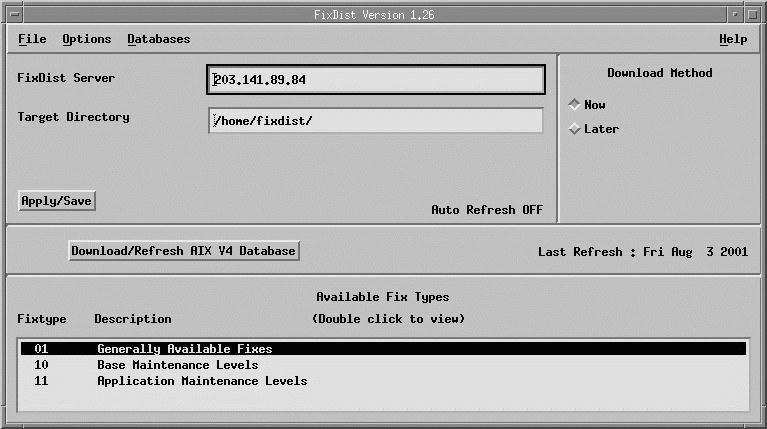
\includegraphics[width=\textwidth]{fixdist.png}
% Esta linea es para el output de BM2FONT
%\centerline{\input{prova}\setprova}
\end{center}
\caption{Interfaz de {\tt fixdist} (AIX).}
\label{fixdist}
\end{figure}
\\Por fortuna, en un sistema AIX podemos utilizar {\tt fixdist}, un c\'omodo
entorno gr\'afico (en la figura \ref{fixdist} podemos ver su interfaz) que
nos facilitar\'a enormente esta tarea, ya que calcula todos los parches que
conformar\'an nuestro \'arbol de prerequisitos y los descarga autom\'aticamente;
gracias a esta herramienta, descargar todos los prerrequisitos de un
determinado parche se convierte en una tarea trivial.
\section{Extensiones de la seguridad: filtros IP}
En versiones m\'as o menos recientes de AIX el operativo proporciona `de serie' unos interesantes mecanismos de seguridad IP basados en t\'uneles y filtros de 
paquetes, algo similar -- guardando las distancias -- a {\tt ipchains} o {\tt
iptables} en Linux; el uso de t\'uneles requiere filtros, pero el de filtros no
necesita para nada los t\'uneles. Para poder utilizar ambos mecanismos 
necesitamos tener instalado el paquete (m\'as concretamente, el {\it fileset}) 
{\tt bos.net.ipsec.rte}:
\begin{quote}
\begin{verbatim}
bruja:/# lslpp -l bos.net.ipsec.rte
  Fileset                      Level  State      Description
  ----------------------------------------------------------------------------
Path: /usr/lib/objrepos
  bos.net.ipsec.rte          4.3.3.0  COMMITTED  IP Security

Path: /etc/objrepos
  bos.net.ipsec.rte          4.3.3.0  COMMITTED  IP Security
bruja:/#
\end{verbatim}
\end{quote}
Un t\'unel define una asociaci\'on entre dos m\'aquinas en las que se han
especificado par\'ametros de seguridad compartidos entre los dos extremos del
t\'unel; el hecho de que se implique a otra m\'aquina hace que, excepto en 
entornos muy homog\'enos -- sistemas AIX -- o en casos concretos, no se suela
utilizar este mecanismo. En cambio, el filtrado de paquetes s\'{\i} que se 
utiliza, ya que proporciona a un entorno aislado una protecci\'on frente a 
otras m\'aquinas sin tener que modificar para nada el operativo o las 
aplicaciones de estas: proporciona un sistema de filtrado sencillo pero 
efectivo en m\'aquinas en las que por cualquier motivo -- dinero, utilizaci\'on,
rendimiento\ldots -- no se pueden implantar otras soluciones cortafuegos m\'as
completas, como {\it CheckPoint Firewall--1} o {\it IBM SecureWay Firewall}. Por
este motivo, en este punto vamos a comentar brevemente algunos aspectos del 
filtrado de paquetes en AIX, sin entrar en el apartado de t\'uneles; si alguien
est\'a interesado en profundizar m\'as en estos mecanismos de seguridad IP para
AIX, puede consultar \cite{kn:ibm97b}.\\
\\Para gestionar este sistema de filtrado podemos utilizar \'ordenes como {\tt
rmfilt}, {\tt mkfilt}, {\tt genfilt} o {\tt lsfilt}; como siempre, es 
recomendable consultar las p\'aginas de ayuda de cada una de ellas, aunque en
este caso m\'as que recomendable podr\'{\i}amos decir {\bf imprescindible}, ya 
que el manejo de los filtros no es ni mucho menos inmediato, y la sintaxis para 
definir reglas es relativamente compleja. Para poner en marcha el sistema de 
filtrado necesitamos generar reglas y posteriormente activarlas; en el fichero 
{\tt /usr/samples/ipsec/filter.sample} tenemos ejemplos de como definir
una regla, un filtro de red, mediante {\tt genfilt}.\\
\\El uso de {\tt genfilt} puede llegar a ser bastante complicado, debido 
principalmente a su sintaxis (como acabamos de decir, es {\bf imprescindible}
consultar su p\'agina de manual). Para definir una regla nueva es obligatorio
indicar al menos el protocolo sobre el que se aplicar\'a (IPv4 o IPv6), as\'{\i}
como el {\it host} o red origen y su m\'ascara correspondiente; el resto de
par\'ametros (destino, puertos de conexi\'on, interfaz de red\ldots) son 
opcionales, aunque como sucede en muchas otras ocasiones, es necesario estar
atento a los valores que el sistema toma por defecto: por simple Ley de Murphy,
ser\'an restrictivos cuando nos interese que sean permisivos y viceversa. Para
hacernos una idea de c\'omo se definen reglas mediante {\tt genfilt}, si por 
ejemplo necesit\'aramos permitir todo el tr\'afico de una red local contra una
m\'aquina AIX situada en ella (192.168.0.10), la orden para lograrlo ser\'{\i}a
similar a:
\begin{quote}
\begin{verbatim}
bruja:/# genfilt -v 4 -a P -s 192.168.0.0 -m 255.255.0.0 -d 192.168.0.10 -M \
> 255.255.255.255 -i all
bruja:/# 
\end{verbatim}
\end{quote}
Aunque no vamos a entrar aqu\'{\i} en detalles de la sintaxis de las reglas, 
veremos al final de este punto un {\it shellscript} como ejemplo de filtrado en
una m\'aquina AIX en el que se incluir\'an algunas definiciones de filtros; en
cualquier caso, como ya hemos dicho, existe un fichero con ejemplos de reglas en
{\tt /usr/samples/ipsec/filter.sample} que podemos consultar para hacernos una
idea de la sintaxis de {\tt genfilt}.\\
\\Para activar el conjunto de reglas de filtrado que hayamos definido 
previamente mediante tenemos que utilizar la orden {\tt mkfilt}; no obstante, 
antes de esto
debemos haber generado los dispositivos especiales {\tt ipsec$\_$v4} e {\tt 
ipsec$\_$v6} (como su nombre indica, el segundo hace referencia a IPv6, mientras
que el primero es relativo al protocolo cl\'asico) en el sistema de ficheros 
utilizando {\tt mkdev}, ya que de lo contrario la activaci\'on no ser\'a 
posible:
\begin{quote}
\begin{verbatim}
bruja:/# mkfilt -v 4
Device ipsec_v4 not found.
Filter activation for IPv4 not performed.
bruja:/# /usr/sbin/mkdev -c ipsec -t 4
ipsec_v4 Available
bruja:/# /usr/sbin/mkdev -c ipsec -t 6
ipsec_v6 Available
bruja:/# 
\end{verbatim}
\end{quote}
Una vez creados ambos ficheros especiales ya podemos activar el {\it ruleset}
definido; por ejemplo, el siguiente {\it shellscript} -- o modificaciones del
mismo -- puede utilizarse para definir un sencillo sistema de filtrado en
nuestra m\'aquina:
\begin{quote}
\begin{verbatim}
bruja:/# cat /etc/filtros
#!/bin/sh
#
# Script para filtrar paquetes en una maquina AIX.
# Antonio Villalon, Noviembre 2001
#
#############
# Eliminamos y deshabilitamos reglas anteriores
#############
/usr/sbin/rmfilt -v 4 -n all
/usr/sbin/rmfilt -v 6 -n all
/usr/sbin/mkfilt -v 4 -d
/usr/sbin/mkfilt -v 6 -d
#############
# Permitimos todo desde LAN
#############
genfilt -v 4 -a P -s 192.168.0.0 -m 255.255.0.0 -d 192.168.0.10 -M \
255.255.255.255 -i all
#############
# Salida, todo abierto
#############
genfilt -v 4 -a P -s 192.168.0.10 -m 255.255.255.255 -d 0 -M 0
#############
# Vuelta de DNS
#############
genfilt -v 4 -a P -s 0 -m 0 -d 0 -M 0 -g N -c udp -o eq -p 53 -O gt -P 1023
#############
# Prohibimos todo lo no habilitado por defecto
#############
genfilt -v 4 -a P -s 0 -m 0 -d 192.168.0.10 -M 255.255.255.255 -c tcp/ack
genfilt -v 4 -a D -s 0 -m 0 -d 192.168.0.10 -M 255.255.255.255 
#############
# Activamos las reglas para IP e IPv6
#############
/usr/sbin/mkfilt -v 4 -u
/usr/sbin/mkfilt -v 6 -u
bruja:/#
\end{verbatim}
\end{quote}
Podemos ver que la activaci\'on del conjunto de reglas se realiza mediante la
opci\'on {\tt `-u'} de {\tt mkfilt}, tanto para IPv4 como para IPv6; esto 
significa que es a partir de la ejecuci\'on de esta orden cuando el sistema de 
filtrado comienza a funcionar.\\
\\Para consultar el conjunto de reglas definidas en nuestra m\'aquina podemos
utilizar el comando {\tt lsfilt} (si lo ejecutamos sin ninguna opci\'on nos
proporcionar\'a el listado de todas las reglas, tanto activas -- las que se 
est\'an aplicando -- como inactivas -- definidas pero sin ser aplicadas --). 
Como en otros sistemas de filtrado, a cada regla se le asigna un n\'umero de
orden, y es ese n\'umero el que indica la precedencia de su aplicaci\'on: si
un paquete hace {\it match} con una cierta regla, es esa la que se aplica, 
descartando las que son posteriores; es una aproximaci\'on similar a la seguida
en {\it Firewall--1} o {\it ipchains}, pero diferente de la de otros cortafuegos
como {\it IP Filter}. Para consultar una regla concreta podemos utilizar las
diferentes opciones de la orden {\tt lsfilt}:
\begin{quote}
\begin{verbatim}
bruja:/# lsfilt -v 4 -n 3
Rule 3:
Rule action         : permit
Source Address      : 192.168.0.0
Source Mask         : 255.255.0.0
Destination Address : 192.168.0.10
Destination Mask    : 255.255.255.255
Source Routing      : yes
Protocol            : all
Source Port         : any 0
Destination Port    : any 0
Scope               : both
Direction           : both
Logging control     : no
Fragment control    : all packets
Tunnel ID number    : 0
Interface           : all
Auto-Generated      : no
bruja:/#
\end{verbatim}
\end{quote}
Para acabar este punto quiz\'as es necesario saber c\'omo deshabilitar el 
sistema de filtrado; ya lo hemos visto antes, en el {\it shellscript} de 
ejemplo, pero hay que recordar que mediante la opci\'on {\tt `-d'} de la orden 
{\tt mkfilt} podemos hacerlo. Esto es especialmente importante en situaciones en
las que un filtro incorrecto deja inaccesible el sistema o alguna aplicaci\'on
cr\'{\i}tica, ya que la posibilidad de deshabilitar todo el filtrado mediante
una orden sencilla, en l\'{\i}nea de comandos, proporciona una soluci\'on 
r\'apida y efectiva este tipo de problemas.
\section{El subsistema de red}
Igual que en Solaris hemos visto, antes de comentar aspectos relativos a la
seguridad del subsistema de red del operativo, la orden {\tt `ndd'}, en AIX es
necesario introducir el comando {\tt `no'} ({\it Network Options}), encargado 
de configurar (y visualizar) par\'ametros del subsistema de red de AIX. Y de la 
misma forma que hemos dicho que la gesti\'on de seguridad de los usuarios 
(contrase\~nas, 
restricciones de acceso, l\'{\i}mites\ldots) es en AIX excelente, y que otros
Unices deber\'{\i}an tomar nota, es justo decir ahora que la configuraci\'on de 
par\'ametros del n\'ucleo relativos a la seguridad en AIX es m\'as pobre que en 
Solaris, aunque no por ello deba considerarse d\'ebil o inadecuada.\\
\\Como en cualquier Unix, una norma b\'asica en la seguridad del subsistema de
red para prevenir ataques de {\it spoofing} es {\bf no} reenviar paquetes a no 
ser que nuestro equipo trabaje como un {\it router} o una pasarela; por tanto, 
es una buena idea desactivar el {\it IP Forwarding} tanto de tramas IP como de
tramas IPv6: 
\begin{quote}
\begin{verbatim}
bruja:/# no -o ipforwarding=0
bruja:/# no -o ip6forwarding=0
bruja:/#
\end{verbatim}
\end{quote}
Para evitar ataques de {\it SYN Flooding} es interesante el par\'ametro {\tt
clean$\_$partial$\_$conns}, que define si se van a eliminar aleatoriamente 
conexiones incompletas (aquellas en las que no se ha completado el protocolo a 
tres bandas) de la cola del servidor para dejar hueco a nuevas entradas:
\begin{quote}
\begin{verbatim}
bruja:/# no -o clean_partial_conns=1
bruja:/#
\end{verbatim}
\end{quote}
Respecto a algunos aspectos del protocolo {\sc icmp}, es recomendable no 
responder a los {\it pings} lanzados a direcciones de {\it broadcast}, ya que 
si lo hacemos podemos llegar a saturar una red, facilitando ataques de 
negaci\'on de servicio; esto se consigue asignando a la directiva {\tt 
bcastping} un valor falso (`0'). De la misma forma, es tambi\'en interesante 
no permitir {\it broadcasts} dirigidos a una pasarela para que sean emitidos en
el otro extremo de la misma, para lo que debemos asignar a {\tt 
directed$\_$broadcast} un valor `0'. Adem\'as podemos hacer que nuestra 
m\'aquina no responda a peticiones {\sc icmp} del tipo {\sc 
icmp$\_$mask$\_$request}, asignando a la directiva {\tt icmpaddressmask} el 
valor `0' (el que tiene por defecto):
\begin{quote}
\begin{verbatim}
bruja:/# no -o bcastping=0
bruja:/# no -o directed_broadcast=0
bruja:/# no -o icmpaddressmask=0
bruja:/#
\end{verbatim}
\end{quote}
Tambi\'en relacionados con el protocolo {\sc icmp}, es necesario comentar 
aspectos relativos a las tramas {\sc icmp$\_$redirect}; podemos restringir la 
emisi\'on de estos paquetes (recordemos que s\'olo un {\it router} deber\'{\i}a
poder enviarlos) mediante la directiva {\tt ipsendredirects}, 
mientras que para deshabilitar la recepci\'on de los mismos podemos utilizar 
{\tt ipignoreredirects}:
\begin{quote}
\begin{verbatim}
bruja:/# no -o ipsendredirects=0
bruja:/# no -o ipignoreredirects=1
bruja:/#
\end{verbatim}
\end{quote}
Como ya vimos, la gesti\'on de paquetes {\it source routed} tambi\'en puede
presentar serias amenazas a nuestra seguridad; en AIX tenemos varios 
par\'ametros relativos al manejo de este tipo de tramas. En primer lugar es
necesario desactivar tanto la generaci\'on como la recepci\'on y el reenv\'{\i}o
de las mismas, mediante los par\'ametros {\tt ipsrcroutesend}, {\tt 
ipsrcrouterecv} e {\tt ipsrcrouteforward} respectivamente, asignandoles a todos 
valores de `0' (falso); el \'ultimo de ellos tiene un equivalente especial para
IPv6 denominado {\tt ip6srcrouteforward}. Adem\'as, 
otro par\'ametro importante es {\tt nonlocsrcroute}, que indica que s\'olo los 
paquetes {\it source routed} estrictos ({\it strict source routed}, paquetes en 
los que se especifica el camino concreto que ha de seguir la trama, a 
diferencia de los paquetes {\it loose source routed}, en los que s\'olo se
marca un nodo por el que la trama ha de pasar y no el camino completo) pueden 
ser reenviados a trav\'es del {\it 
host}; su valor tambi\'en ha de ser falso\footnote{En sistemas {\sc SP/2}
({\it Scallable Power Parallel}) de IBM esto puede ser problem\'atico para 
algunas aplicaciones, por lo que es conveniente consultar la documentaci\'on
del sistema en cada caso.}:
\begin{quote}
\begin{verbatim}
bruja:/# no -o ipsrcroutesend=0
bruja:/# no -o ipsrcrouterecv=0
bruja:/# no -o ipsrcrouteforward=0
bruja:/# no -o ip6srcrouteforward=0
bruja:/# no -o nonlocsrcroute=0
bruja:/#
\end{verbatim}
\end{quote}
Respecto al {\it timeout} de la cach\'e {\sc arp} del que ya hemos hablado en
Solaris y Linux, en AIX este par\'ametro viene definido por la variable {\tt
arpt$\_$killc}; no obstante, su valor afecta tanto a entradas {\sc arp} no
utilizadas como a entradas activas, por lo que nos debemos plantear con cuidado
la conveniencia de modificarlo; en cualquier caso, podemos definir en minutos
el {\it timeout} tambi\'en mediante la orden {\tt no}:
\begin{quote}
\begin{verbatim}
bruja:/# no -o arpt_killc=1
bruja:/#
\end{verbatim}
\end{quote}
Adem\'as de la orden {\tt `no'}, otro comando que nos permite configurar 
par\'ametros interesantes para nuestra seguridad a nivel del subsistema de red
-- especialmente si administramos un servidor {\sc nfs} -- es {\tt `nfso'}, que
configura y visualiza diferentes par\'ametros relacionados con este sistema de
ficheros; su sintaxis es bastante similar a la de {\tt `no'} (en cualquier caso,
como sucede con todas las \'ordenes de un sistema Unix, es recomendable 
consultar la p\'agina de manual correspondiente), y entre los par\'ametros que
permite configurar existen tambi\'en algunos relacionados con la seguridad del
sistema. Quiz\'as el m\'as importante es {\tt portcheck}, que define el 
comportamiento del servidor ante peticiones provenientes de puertos no 
privilegiados: si su valor es 0 (por defecto es as\'{\i}) no se efect\'ua
ning\'un tipo de comprobaci\'on, mientras que si es 1 se realiza el {\it port
checking} y s\'olo se admiten peticiones desde puertos remotos privilegiados;
por ejemplo, si queremos que esto sea as\'{\i} debemos ejecutar la siguiente
orden (recordamos que, al igual que suced\'{\i}a con {\tt `no'}, los cambios
s\'olo tienen efecto sobre el {\it kernel} que se encuentra en ejecuci\'on, por
lo que si se produce un reinicio de la m\'aquina el comportamiento ser\'a el
definido por defecto):
\begin{quote}
\begin{verbatim}
bruja:/# nfso -o portcheck
portcheck= 0
bruja:/# nfso -o portcheck=1
bruja:/# nfso -o portcheck
portcheck= 1
bruja:/# 
\end{verbatim}
\end{quote}
Existen otros par\'ametros configurables mediante {\tt nfso} que nos pueden
resultar interesantes para incrementar nuestra seguridad; por ejemplo, {\tt
nfs$\_$use$\_$reserve$\_$ports} puesto a 0 (por defecto) especificar\'a que se 
utilicen puertos no reservados para las comunicaciones entre cliente y servidor
{\sc nfs}, {\tt nfs$\_$max$\_$connections} y {\tt nfs$\_$max$\_$threads} definen
respectivamente l\'{\i}mites al n\'umero de conexiones simult\'aneas y de hilos 
servidores que se van a aceptar en un sistema AIX, etc. Como siempre, es 
imprescindible consultar la p\'agina de manual correspondiente en la versi\'on
de AIX que estemos ejecutando para conocer todos los par\'ametros sintonizables
mediante {\tt `nfso'} y sus repercusiones en nuestra seguridad.\\
\\Tal y como suced\'{\i}a con {\tt `ndd'}, los cambios efectuados con {\tt 
`no'} tienen efecto sobre el {\it kernel} que se est\'a ejecutando en un cierto 
momento, por lo que si el sistema se reinicia deberemos volver a dar el valor 
que nos interese a ciertos par\'ametros ejecutando la orden en el arranque de 
la m\'aquina. En AIX este arranque es m\'as peculiar que en otros entornos, y
si queremos a\~nadir estas instrucciones en cada inicio del sistema debemos 
crear el {\it script} correspondiente y planificarlo para que se ejecute desde 
{\tt /etc/inittab} (\cite{kn:bha01}):
\begin{quote}
\begin{verbatim}
bruja:/# cat /etc/rc.securenet
/usr/sbin/no -o ipforwarding=0
/usr/sbin/no -o ip6forwarding=0
/usr/sbin/no -o clean_partial_conns=1
/usr/sbin/no -o bcastping=0
/usr/sbin/no -o directed_broadcast=0
/usr/sbin/no -o icmpaddressmask=0
/usr/sbin/no -o ipsendredirects=0
/usr/sbin/no -o ipignoreredirects=1
/usr/sbin/no -o ipsrcroutesend=0
/usr/sbin/no -o ipsrcrouterecv=0
/usr/sbin/no -o ipsrcrouteforward=0
/usr/sbin/no -o ip6srcrouteforward=0
/usr/sbin/no -o arpt_killc=1
/usr/sbin/nfso -o portcheck=1
bruja:/# chmod 700 /etc/rc.securenet
bruja:/# mkitab "rcsecurenet:2:once:/etc/rc.securenet 2>&1 >/dev/console"
bruja:/#
\end{verbatim}
\end{quote}
